\documentclass[10pt]{beamer}
\usepackage{uglibeamer2}
%\usepackage{animate}
\title{Structures de données : Pile}
\subtitle{Chapitre 12}
\author{NSI2}

\setminted{fontsize=\small}


\begin{document}
	\maketitle

\begin{frame}{Principe}
	\only<1>{\begin{center}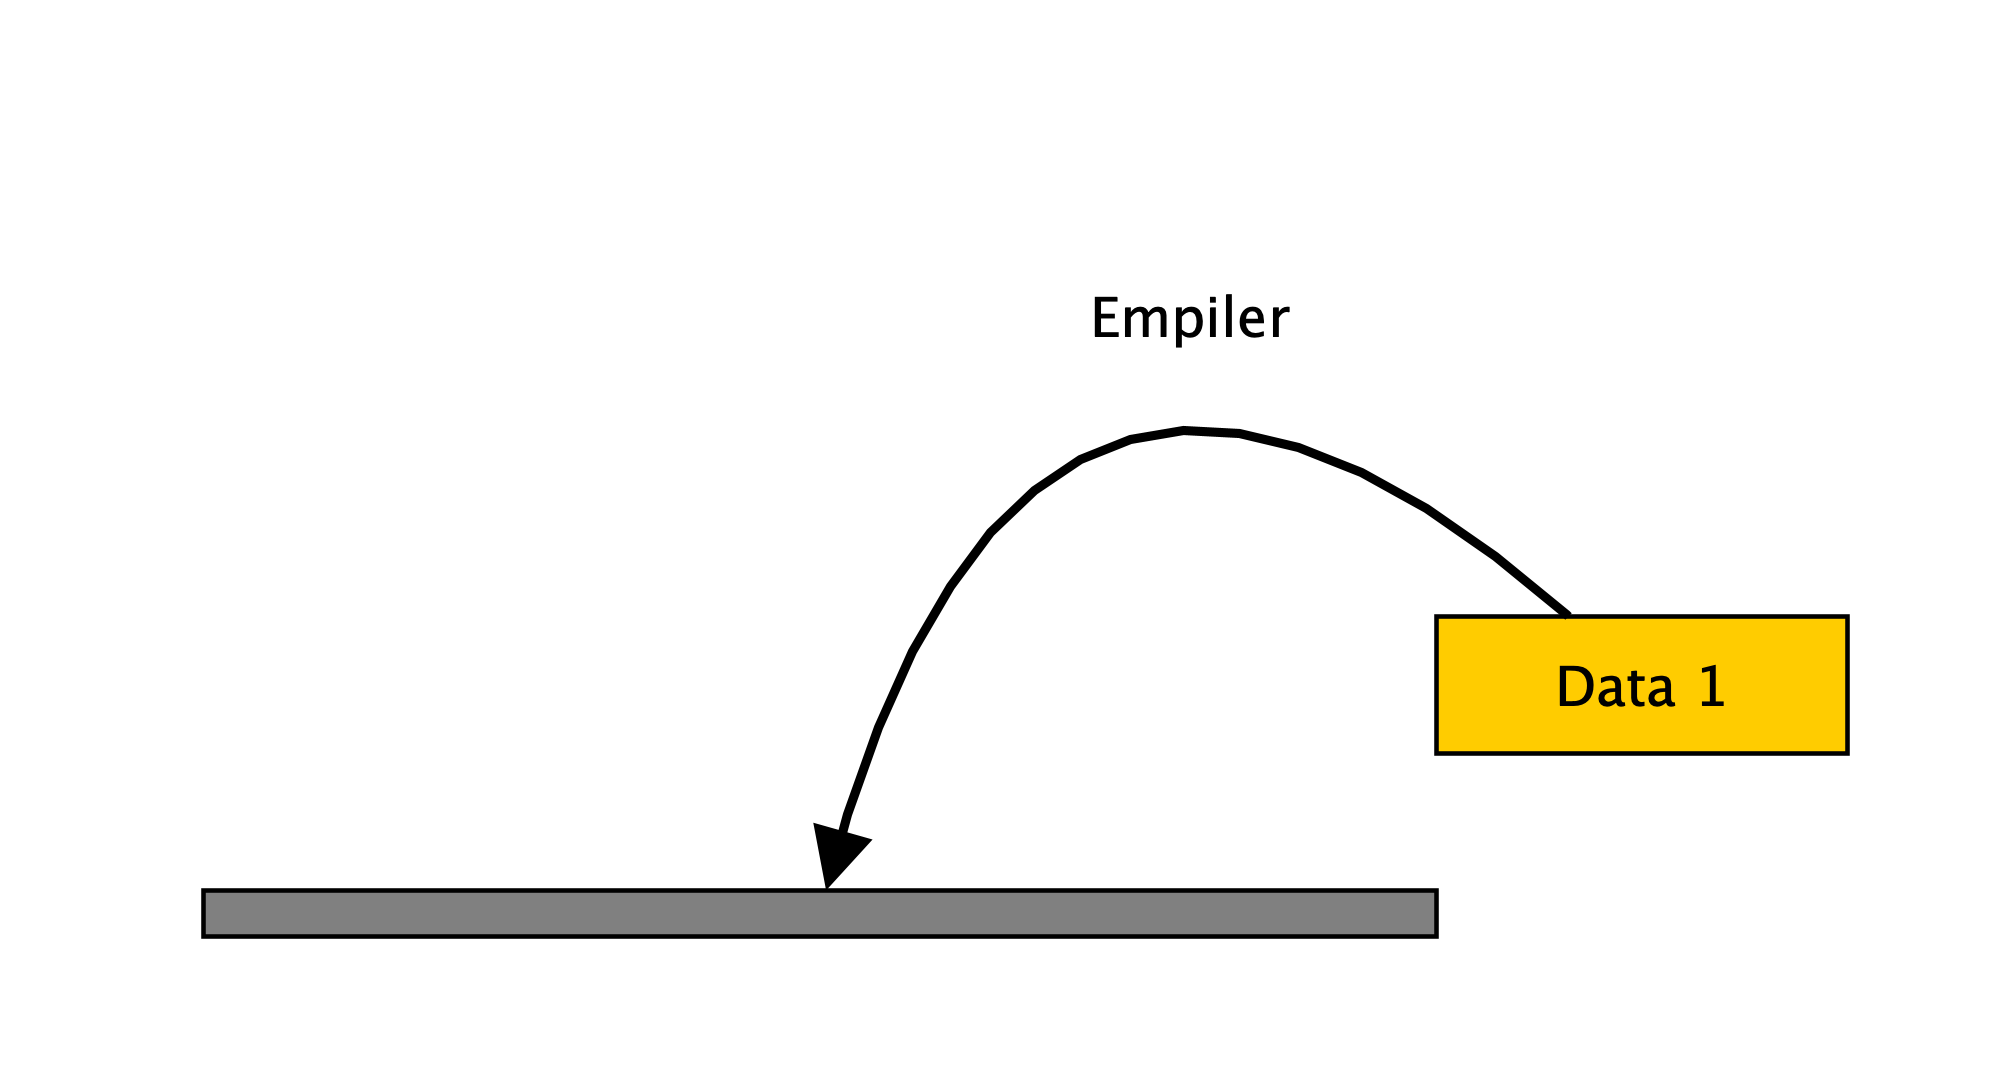
\includegraphics[width=6cm]{img/stack0}\end{center}On part d'une structure vide... }
	\only<2>{\begin{center}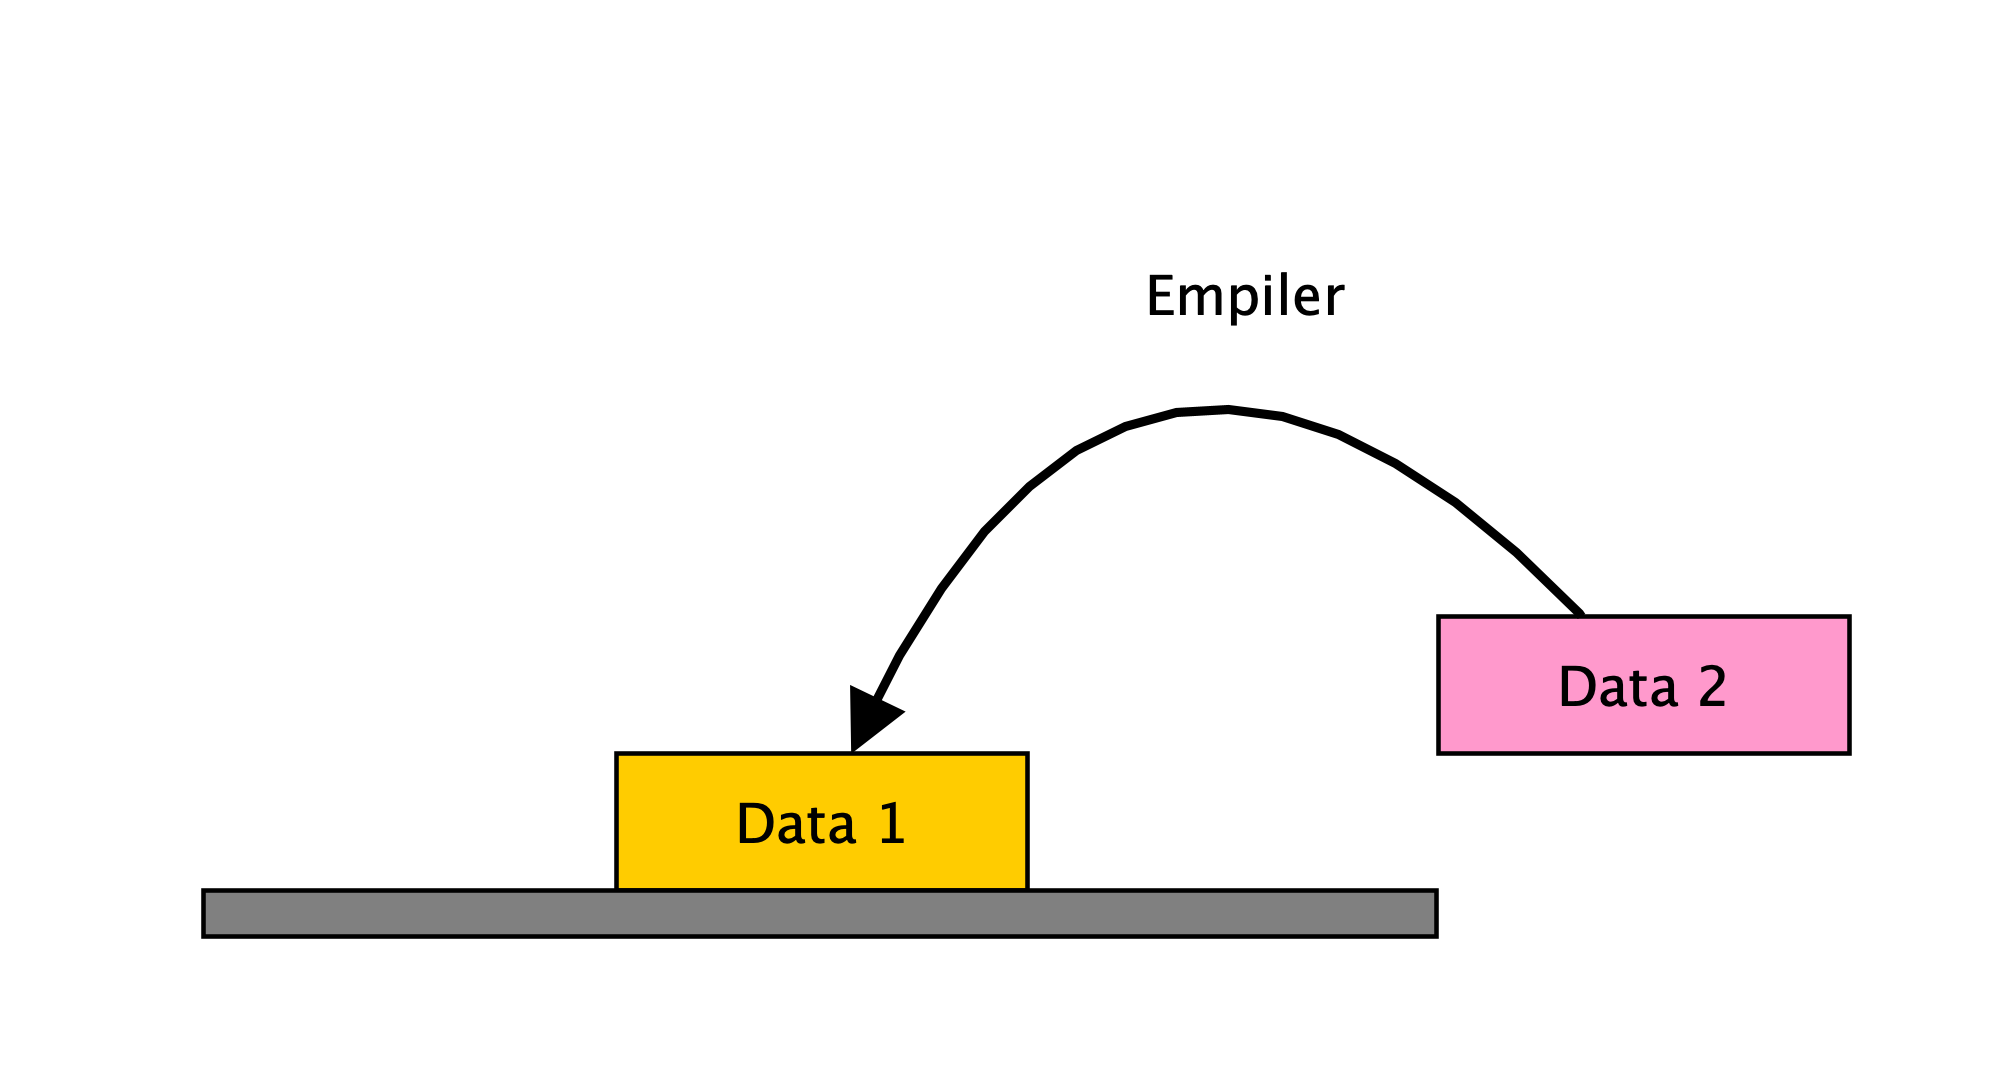
\includegraphics[width=6cm]{img/stack1}\end{center}Sur laquelle on peut empiler... }
	\only<3>{\begin{center}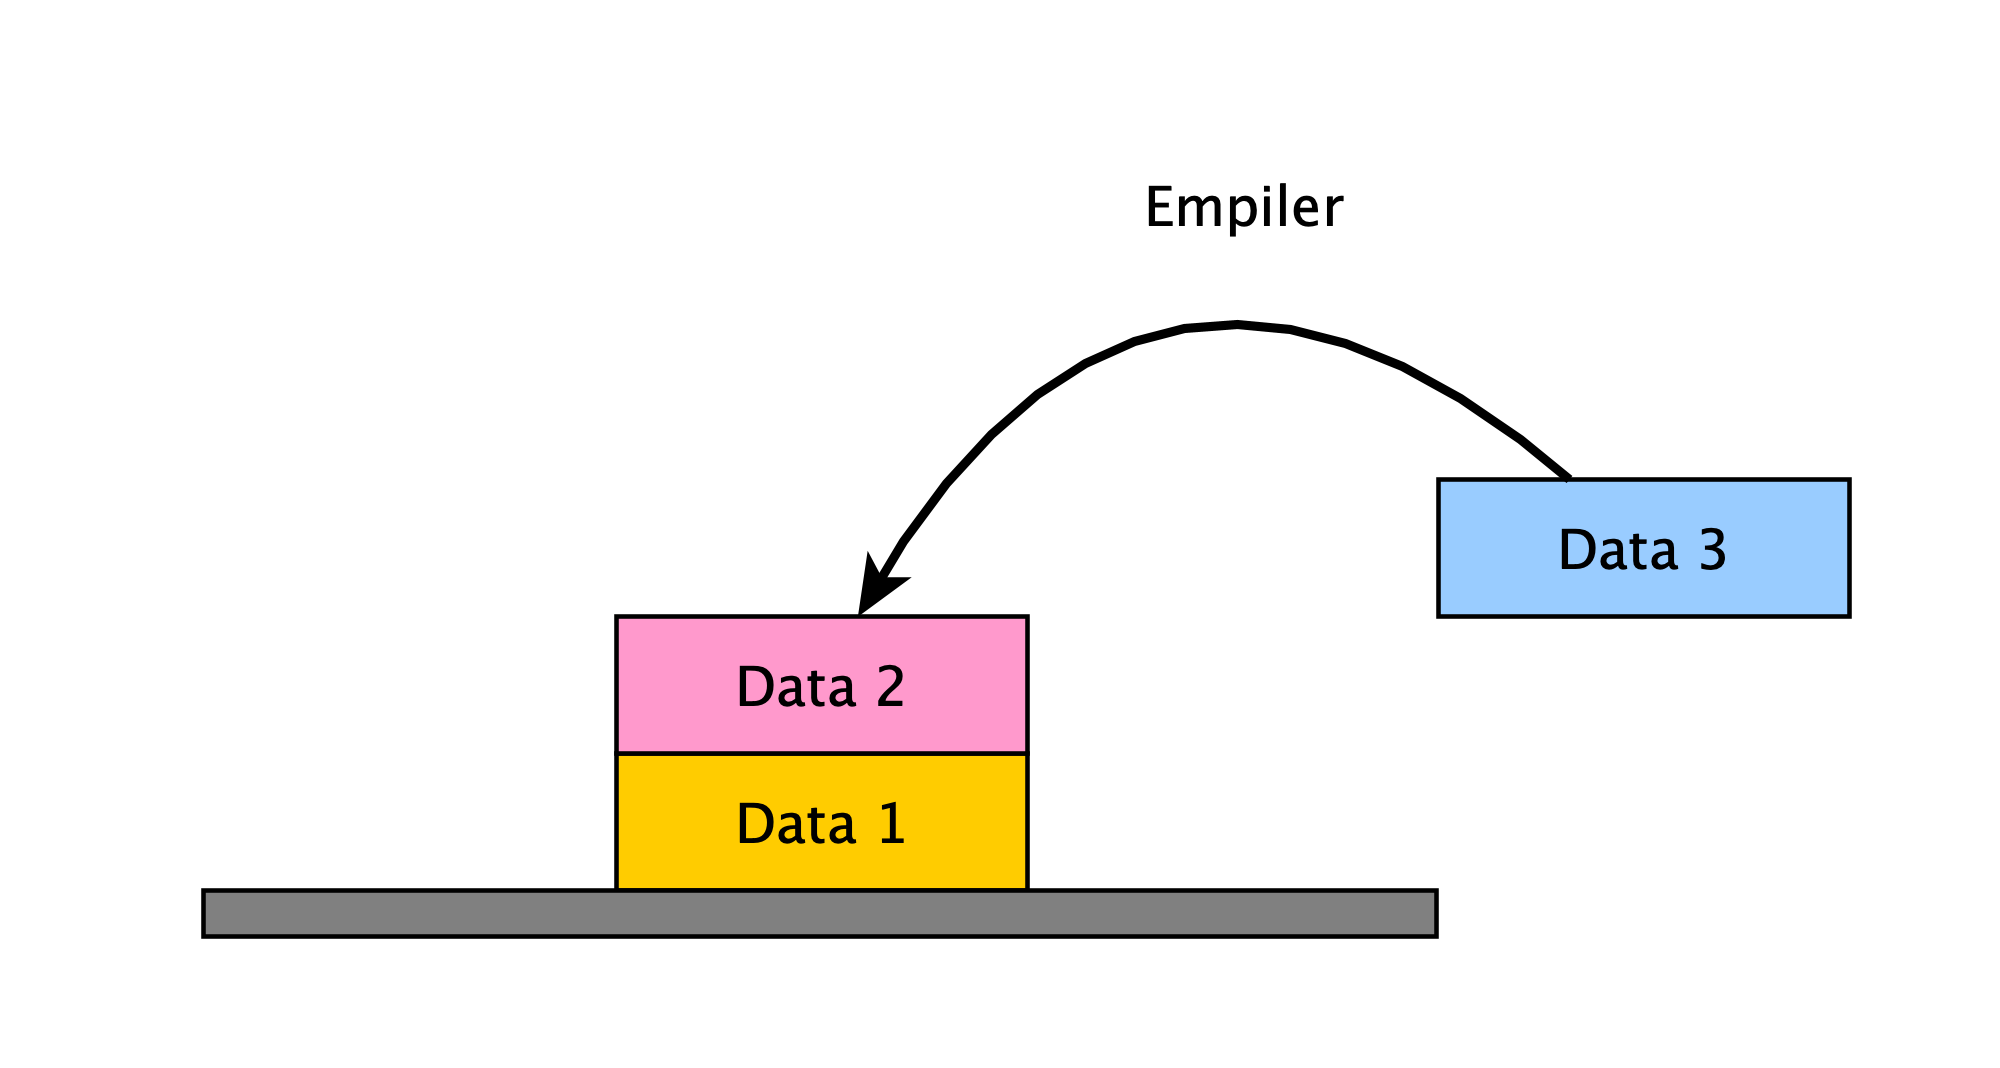
\includegraphics[width=6cm]{img/stack2}\end{center}Au fur et à mesure. }
	\only<4>{\begin{center}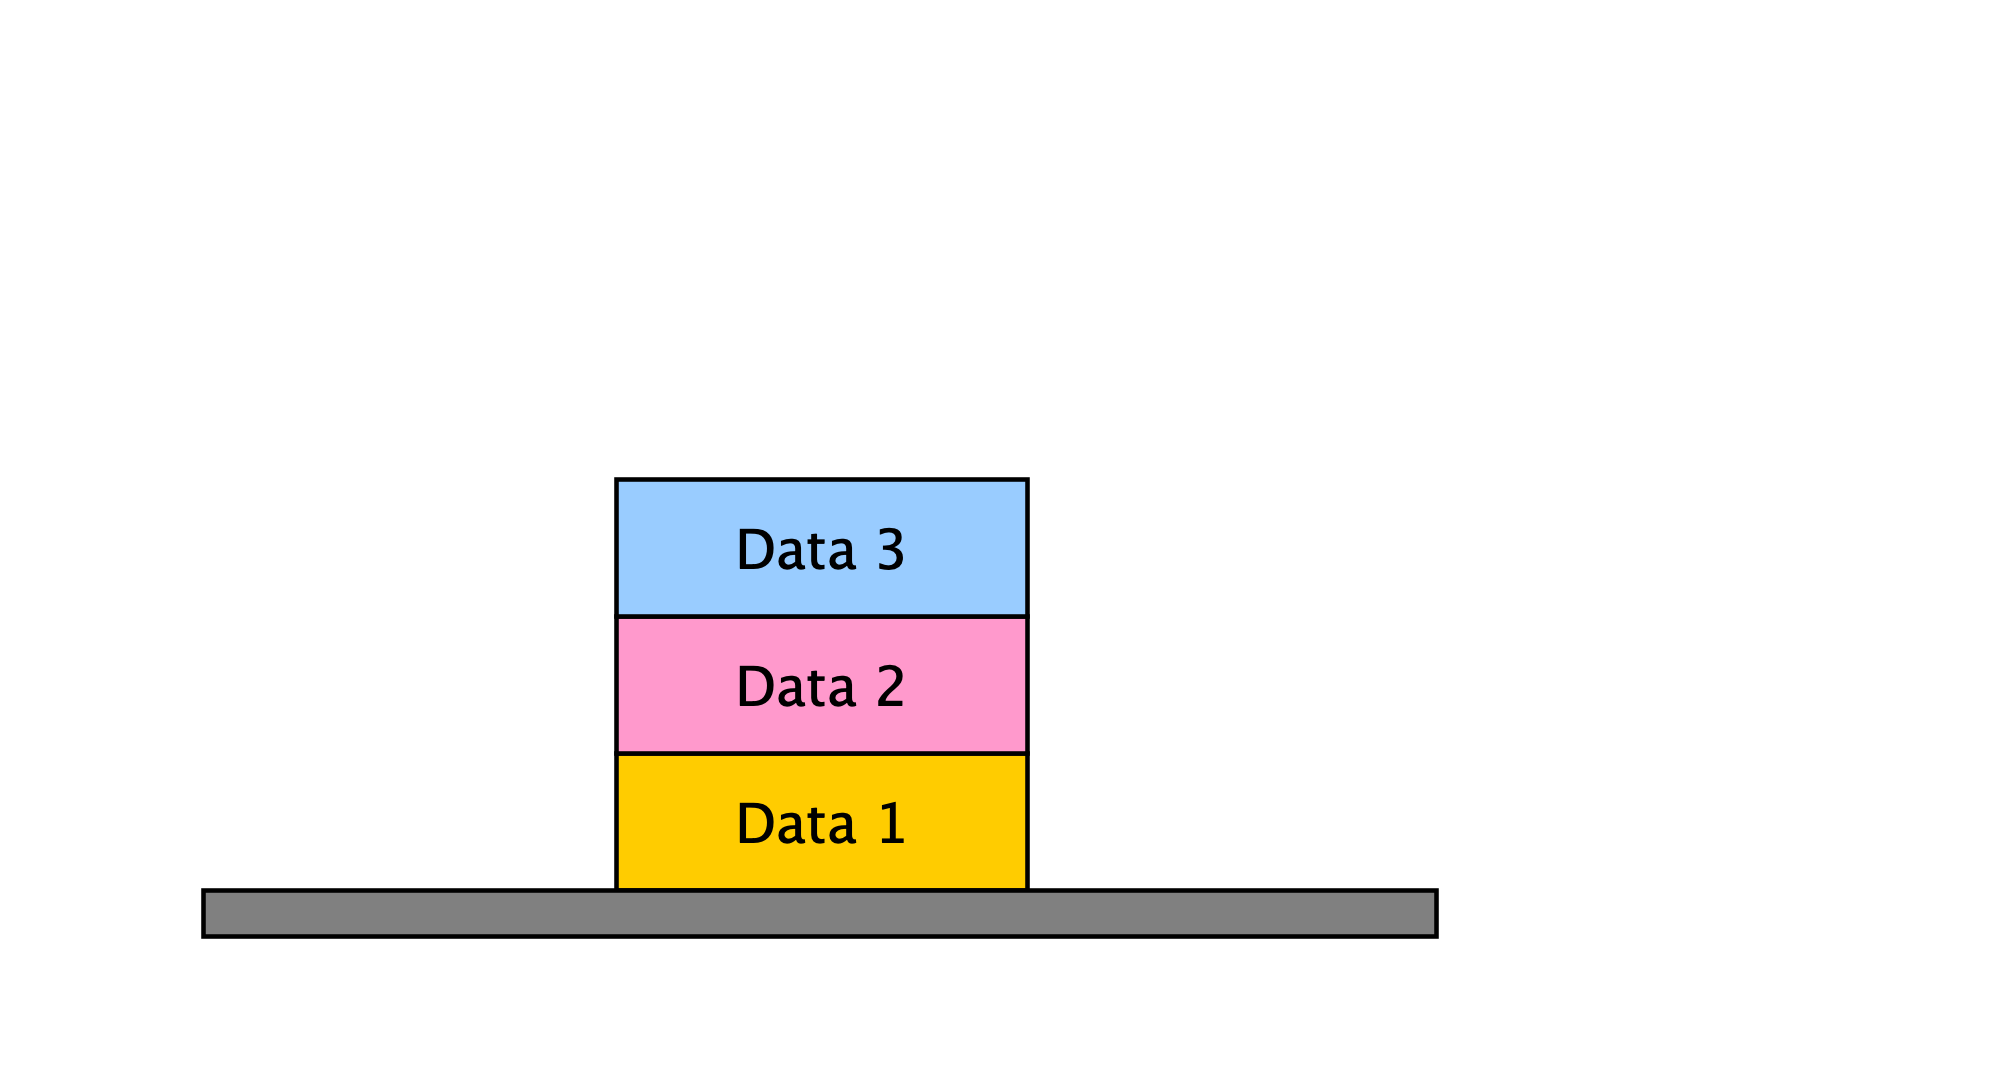
\includegraphics[width=6cm]{img/stack3}\end{center}Seul le dernier élément est accessible. }
	\only<5>{\begin{center}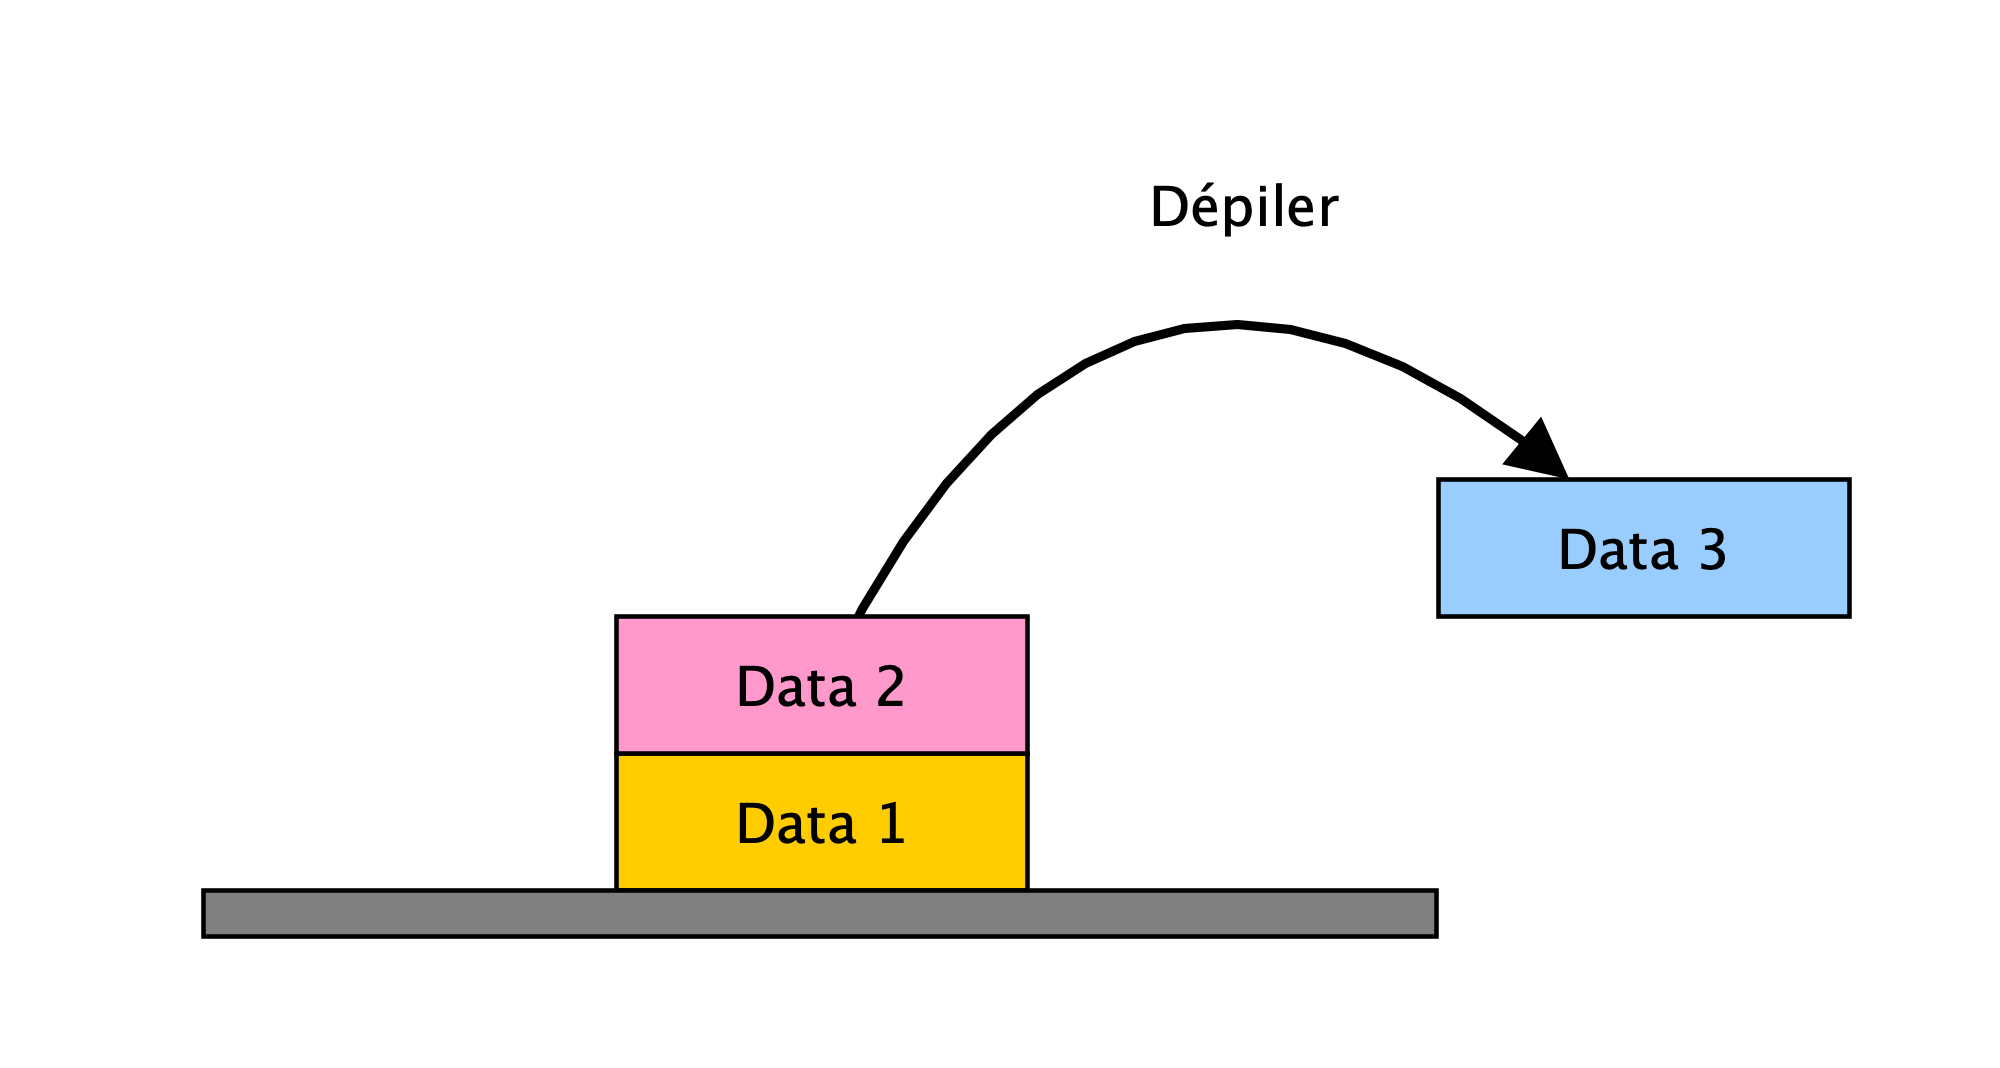
\includegraphics[width=6cm]{img/stack4}\end{center}On peut dépiler. }
	\only<6>{\begin{center}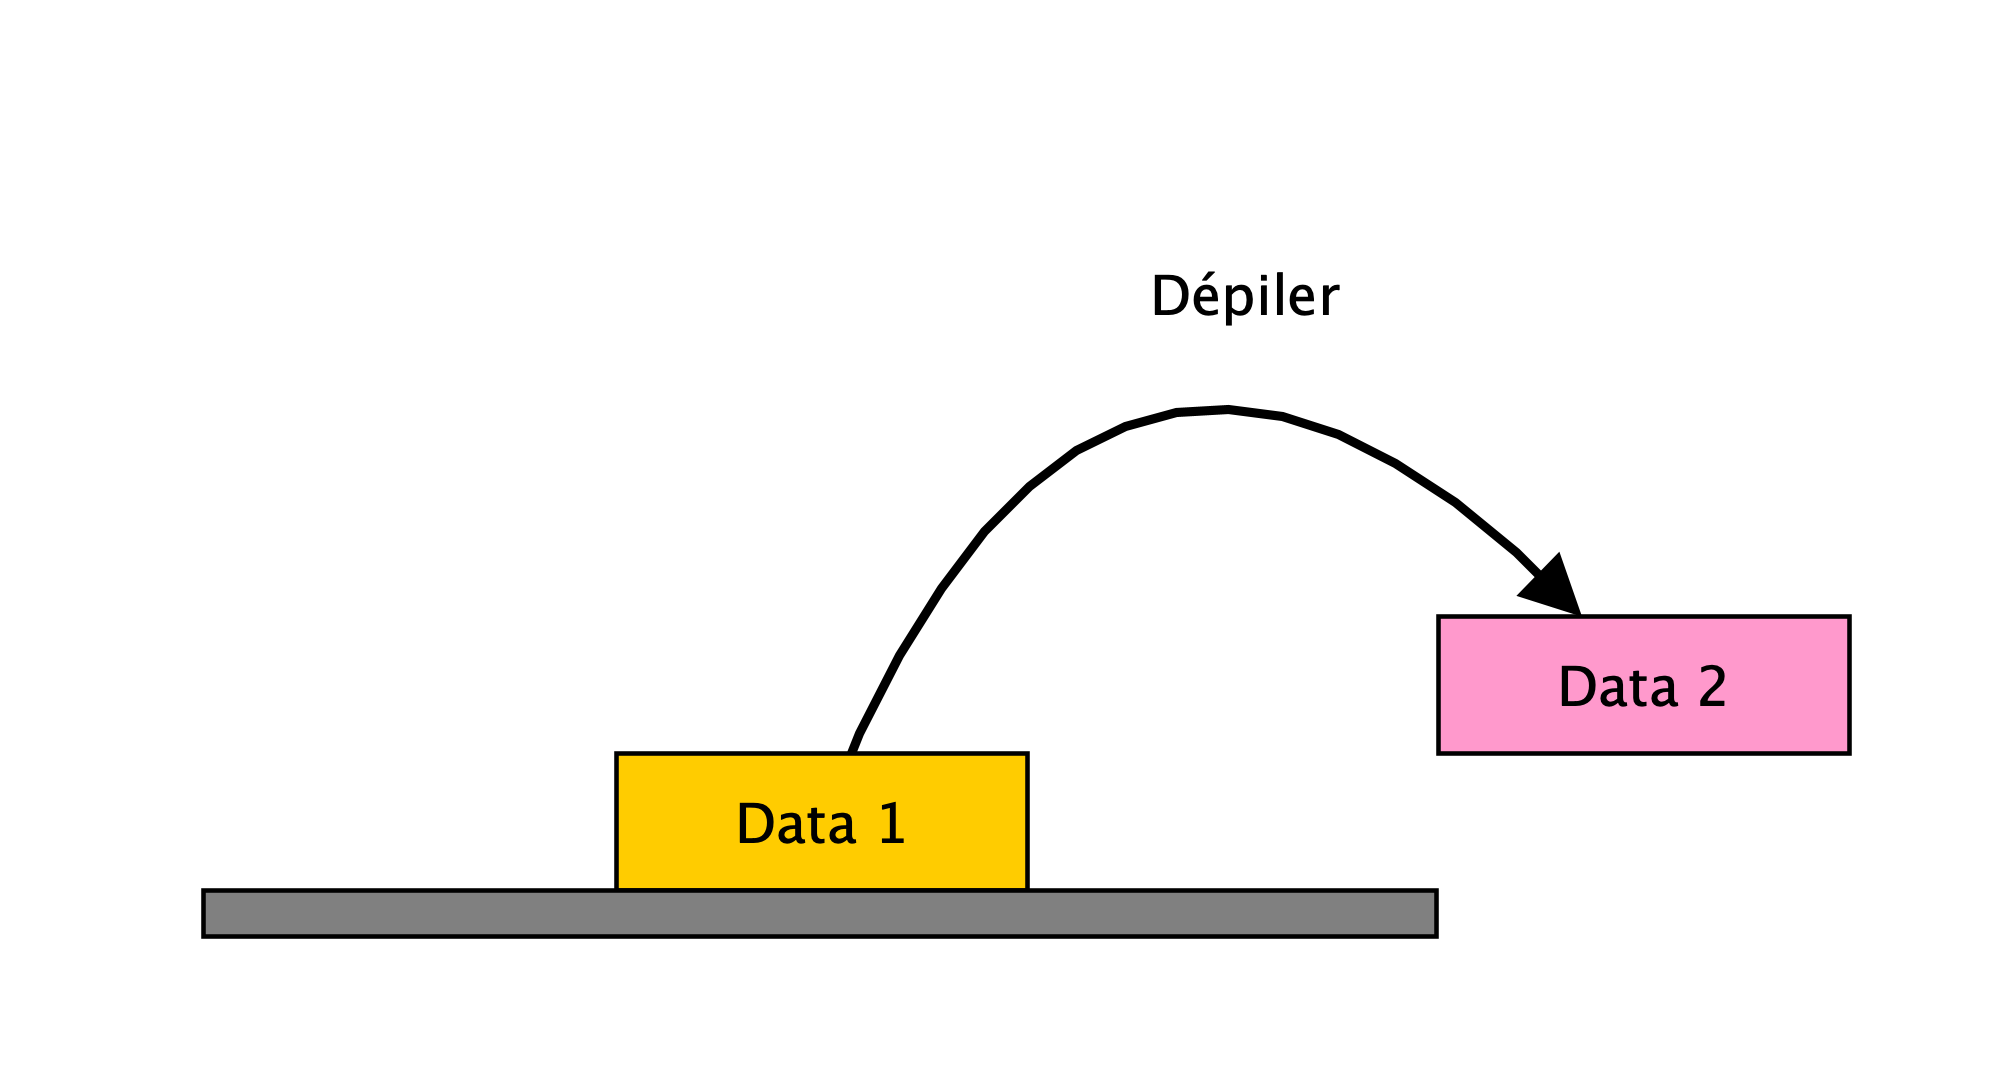
\includegraphics[width=6cm]{img/stack5}\end{center}Les dernières valeurs empilées sont les premières dépilées. }
	\only<7>{\begin{center}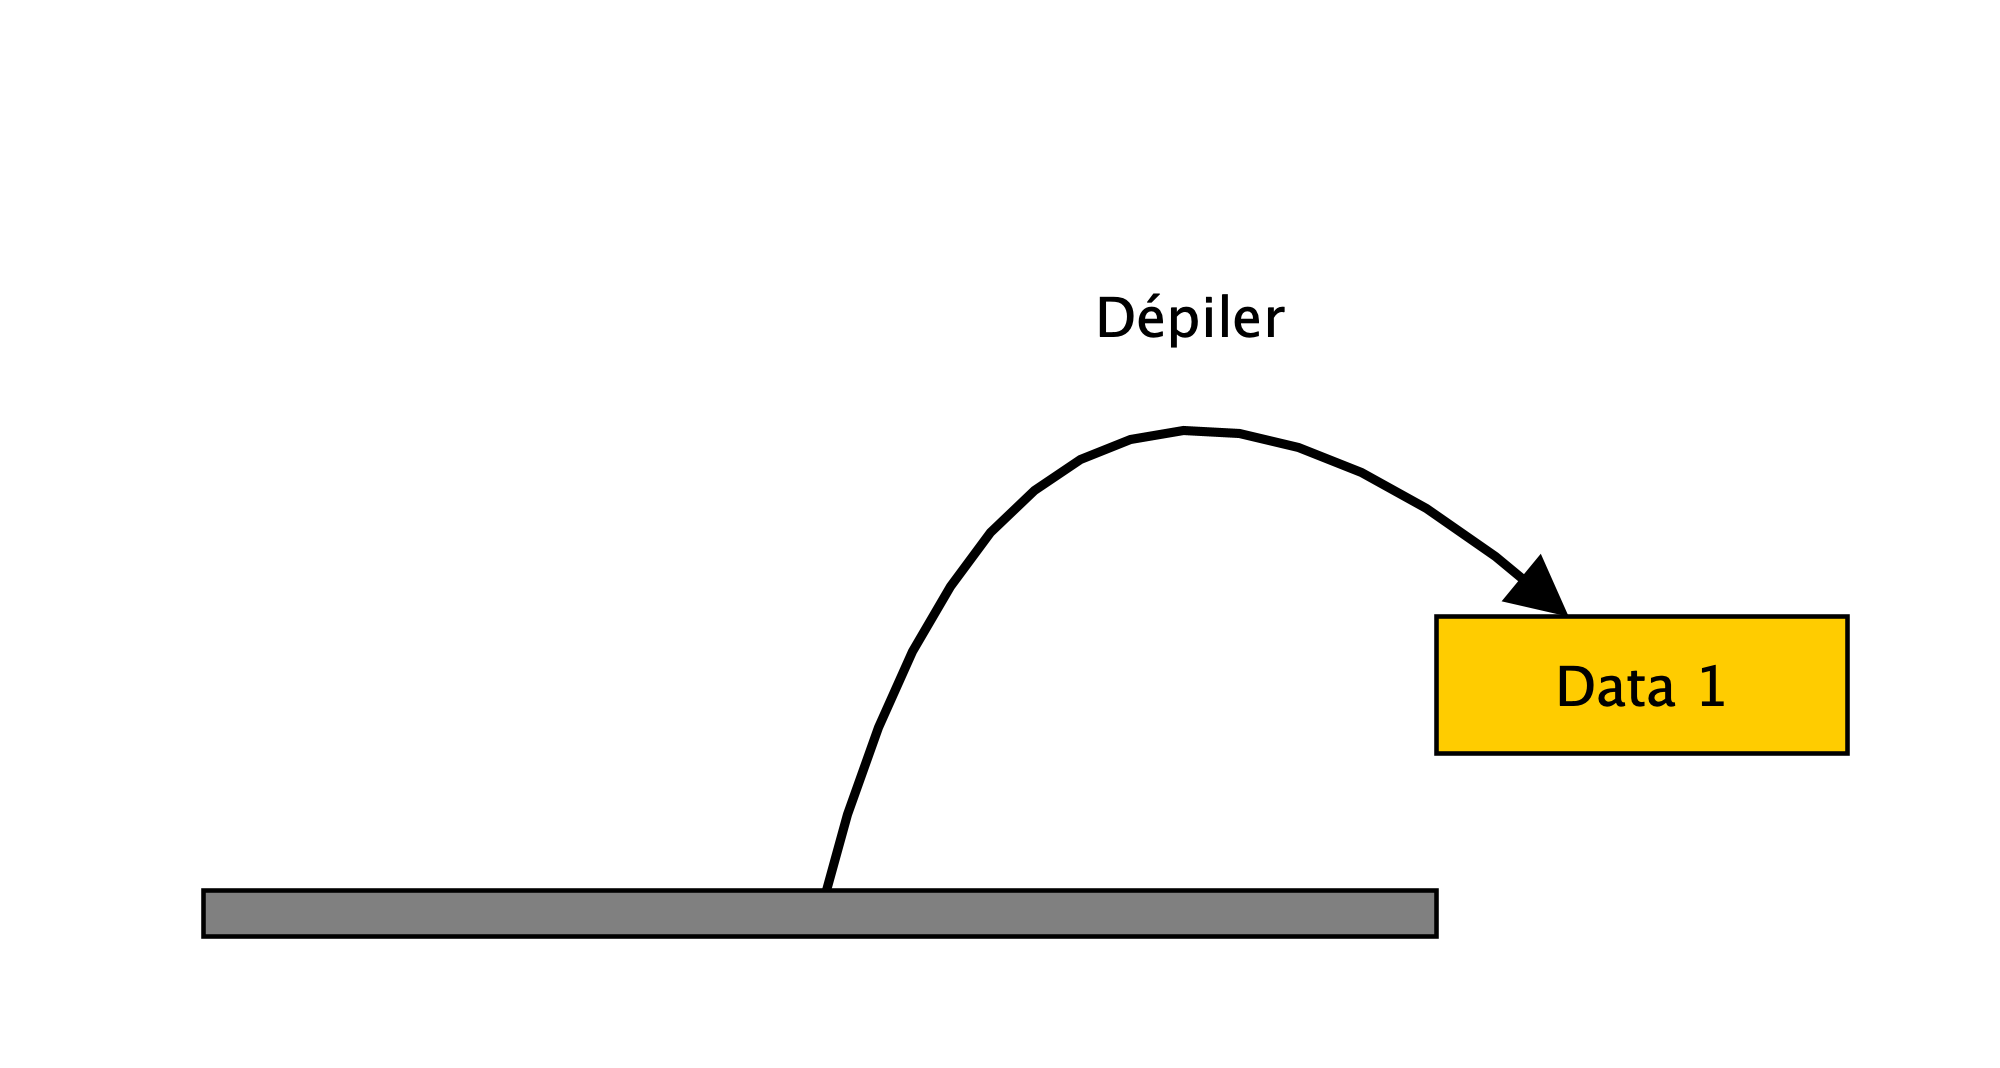
\includegraphics[width=6cm]{img/stack6}\end{center}On parle de LIFO (\textit{Last In First Out}). }
\end{frame}
\begin{frame}{Applications}\pause
	\begin{itemize}
		\item 	Lors de la navigation sur le web, on peut considérer que les liens sont sauvegardés sur une pile par le navigateur.\pause
		\item 	De même pour les logiciels qui utilisent la fonction \texttt{annuler} (le fameux \texttt{CTRL+Z}).\pause
		\item	Lors d'appels de fonctions, les états-mémoires sont sauvegardés sur une pile (notamment lors d'appels récursifs, on l'a déjà vu).\pause
		\item 	Des piles sont utilisées dans divers algorithmes, notamment pour parcourir un arbre « en profondeur ».\pause
		\item 	D'autres applications sont données en exercice.
	\end{itemize}
\end{frame}
\begin{frame}{Interface de la structure de données pile}
	Elle est très simple !\pause
	\begin{itemize}
		\item \textit{pile\_vide()} créée une pile vide\pause
		\item \textit{empiler(pile,valeur)} empile la valeur sur la pile\pause
		\item  \textit{depiler(pile)} renvoie la valeur sur la pile et l'enlève de la pile\pause
		\item \textit{est\_vide()} indique si la pile est vide on non	 
	\end{itemize}
\end{frame}
\begin{frame}[fragile]{Implémentations}
	\begin{itemize}
		\item Simple liste python..\pause
		\item Liste encapsulée dans un objet.\pause
		\item Listes imbriquées :\\
\begin{minted}{python}
[]
[1] # on a empilé 1
[2, [1]] # puis 2
[3, [2, [1]]] # puis 3
...
\end{minted}
	\end{itemize}
\end{frame}
\begin{frame}[fragile]{Implémentation objet}
\begin{minted}{python}
class Stack:
    def __init__(self):
        """ Creates an empty stack """
        self.content = []
        
    def is_empty(self) -> bool:
        """ Indicates whether the stack's empty or not """
        return self.content == []
\end{minted}
\end{frame}

\begin{frame}[fragile]{Implémentation objet (suite et fin)}
	\begin{minted}{python}
    def push(self, value):
        """ Pushes the value on the top of the stack """
        self.content.append(value)

    def pop(self):
        """ Retrieves the value from the top of the stack """
        if self.is_empty():
            raise IndexError('Stack Empty')
        return self.content.pop()
	\end{minted}
\end{frame}
\end{document}